\documentclass[11pt,a4paper]{article}

% ============================================================
% Paquetes
% ============================================================
\usepackage[utf8]{inputenc}
\usepackage[T1]{fontenc}
\usepackage[spanish,es-tabla]{babel}
\usepackage[a4paper,margin=2.5cm]{geometry}
\usepackage{graphicx}
\usepackage{booktabs}
\usepackage{array}
\usepackage{tabularx}
\usepackage{caption}
\usepackage{subcaption}
\usepackage{xcolor}
\usepackage{hyperref}
\usepackage{listings}
\usepackage{amsmath}
\usepackage{enumitem}
\usepackage{fancyhdr}
\usepackage{titlesec}

% ============================================================
% Hyperlinks
% ============================================================
\hypersetup{
    colorlinks=true,
    linkcolor=blue!60!black,
    urlcolor=blue!60!black,
    citecolor=blue!60!black,
    pdftitle={Detección de Cumplimiento de EPP con YOLOv8},
    pdfauthor={Jesús Percy Nazario Portilla},
}

% ============================================================
% Listings (código)
% ============================================================
\definecolor{codegray}{rgb}{0.95,0.95,0.95}
\definecolor{codekeyword}{rgb}{0.13,0.29,0.53}
\definecolor{codestring}{rgb}{0.31,0.60,0.02}
\definecolor{codecomment}{rgb}{0.50,0.50,0.50}

\lstset{
    backgroundcolor=\color{codegray},
    basicstyle=\ttfamily\footnotesize,
    keywordstyle=\color{codekeyword}\bfseries,
    stringstyle=\color{codestring},
    commentstyle=\color{codecomment}\itshape,
    breaklines=true,
    frame=single,
    numbers=left,
    numberstyle=\tiny\color{codecomment},
    showstringspaces=false,
    tabsize=2,
    language=Python,
}

% ============================================================
% Encabezados
% ============================================================
\pagestyle{fancy}
\fancyhf{}
\fancyhead[L]{\small Detección de Cumplimiento de EPP — YOLOv8}
\fancyhead[R]{\small \thepage}
\renewcommand{\headrulewidth}{0.4pt}

\titleformat{\section}{\normalfont\Large\bfseries}{\thesection.}{0.5em}{}
\titleformat{\subsection}{\normalfont\large\bfseries}{\thesubsection}{0.5em}{}

% ============================================================
% Información del documento
% ============================================================
\title{
    \vspace{-1.5cm}
    \rule{\linewidth}{0.5pt}\\[0.5cm]
    {\Huge \bfseries Detección de Cumplimiento de Normas\\ de Seguridad en Obras de Construcción}\\[0.3cm]
    {\Large Parcial — Deep Learning aplicado a visión por computadora}\\[0.3cm]
    \rule{\linewidth}{0.5pt}
}
\author{Jesús Percy Nazario Portilla}
\date{\today}

% ============================================================
% Documento
% ============================================================
\begin{document}

\maketitle
\thispagestyle{empty}

\vspace{1cm}
\begin{center}
\textbf{Repositorio:} \url{https://github.com/PercyTechX/epp-yolo-compliance}\\[0.3em]
\textbf{Modelo final (Release v1.0):} \url{https://github.com/PercyTechX/epp-yolo-compliance/releases/tag/v1.0}
\end{center}

\vspace{1cm}

\begin{abstract}
\noindent Se entrenó un detector YOLOv8s para identificar trabajadores de
construcción y los elementos de protección personal (EPP) que portan, y se
acopló un módulo determinista de verificación de cumplimiento. El modelo
final alcanza \textbf{mAP@0.5 = 0.771} sobre un conjunto de prueba no
visto (3.895 imágenes), con desempeño excelente en las tres clases
críticas (cabeza con casco, cabeza sin casco y chaleco, todas con
mAP@0.5 $\geq$ 0.947). Durante el desarrollo se identificó una limitación
importante derivada de la combinación de tres datasets con anotación
parcial no superpuesta: el modelo predice clases distintas según el
``estilo'' de la imagen, lo que limita la emisión de veredictos
CONFORME cuando se evalúa por trabajador. Esta limitación se documenta
cuantitativamente y se valida experimentalmente comparando contra un
modelo externo entrenado sobre un dataset con anotación completa, que
produce 2.75$\times$ más veredictos definitivos sobre la misma escena.
\end{abstract}

\newpage
\tableofcontents
\newpage

% ============================================================
\section{Introducción}
% ============================================================

\subsection{Problema}

Las obras de construcción son entornos de alto riesgo. El uso correcto del
casco de seguridad y del chaleco reflectivo es una de las medidas más
básicas para reducir la tasa de accidentes. La supervisión manual del
cumplimiento de estas normas es costosa, intermitente y susceptible a
sesgos humanos.

Este trabajo aborda el problema de \textbf{detectar automáticamente
trabajadores y clasificar su estado de cumplimiento del EPP} a partir de
imágenes y video de obras, abordando tres desafíos técnicos centrales:

\begin{enumerate}
    \item \textbf{Oclusión severa}: trabajadores parcialmente ocultos por
    maquinaria, andamios u otros trabajadores.
    \item \textbf{Detección de objetos pequeños}: trabajadores lejanos con
    pocos píxeles en la imagen.
    \item \textbf{Desbalance de clases}: los casos no conformes (la clase
    crítica) son típicamente escasos en grabaciones reales.
\end{enumerate}

\subsection{Objetivos}

\begin{itemize}
    \item Entrenar y evaluar un modelo YOLO ajustado al dominio.
    \item Implementar un verificador de cumplimiento basado en reglas
    como posprocesamiento determinista.
    \item Documentar de forma justificada las decisiones de entrenamiento.
    \item Evaluar cuantitativamente con desglose por clase y nivel de
    oclusión.
    \item Demostrar el sistema sobre video real no visto en entrenamiento.
    \item Reflexionar sobre las implicaciones éticas.
\end{itemize}

\subsection{Estrategia general}

Se adopta una arquitectura híbrida \textbf{percepción + decisión}:

\begin{itemize}
    \item \textbf{Percepción}: un modelo YOLOv8 detecta cabezas
    (con/sin casco), chalecos y cuerpos completos cuando es posible.
    \item \textbf{Decisión}: un módulo Python independiente toma las
    detecciones y emite un veredicto por trabajador (CONFORME /
    NO\_CONFORME / INDETERMINADO).
\end{itemize}

Esta separación es un \textbf{requisito explícito del enunciado} y favorece
la auditabilidad (la lógica de cumplimiento es código legible) y la
modificabilidad (se pueden cambiar reglas sin reentrenar el modelo).

% ============================================================
\section{Datos}
% ============================================================

\subsection{Fuentes}

Se combinaron tres datasets públicos de Roboflow Universe, descargados
en formato YOLOv8:

\begin{table}[h]
\centering
\begin{tabular}{lrll}
\toprule
\textbf{Dataset} & \textbf{Imágenes} & \textbf{Aporta} & \textbf{Licencia} \\
\midrule
Hard Hat Workers & 7.035 & cabezas + person & Public Domain \\
Safety Helmet (lisa-group-de) & 7.035 & cabezas + person & CC BY 4.0 \\
Safety Vest PPE & 11.906 & chalecos & CC BY 4.0 \\
\midrule
\textbf{Total} & \textbf{25.976} & & \\
\bottomrule
\end{tabular}
\caption{Datasets de origen combinados.}
\end{table}

\subsection{Taxonomía unificada}

Las clases de cada dataset original se remapearon a una taxonomía común
de 5 clases mediante una tabla declarativa versionada
(\texttt{configs/class\_mapping.yaml}):

\begin{table}[h]
\centering
\begin{tabular}{rll}
\toprule
\textbf{id} & \textbf{Clase} & \textbf{Significado} \\
\midrule
0 & head\_with\_helmet & Cabeza con casco visible \\
1 & head\_without\_helmet & Cabeza sin casco (clase crítica) \\
2 & person & Cuerpo completo o parcial \\
3 & vest & Chaleco reflectivo visible \\
4 & no\_vest\_person & Persona sin chaleco identificable \\
\bottomrule
\end{tabular}
\caption{Taxonomía unificada de 5 clases.}
\end{table}

\subsection{Splits estratificados}

Se generaron splits \textbf{70/15/15} train/val/test estratificados por
\textbf{combinación de clases presentes en cada imagen}. Esto preserva
la proporción de cada clase en cada split y previene la fuga de datos
entre splits.

\begin{figure}[h]
\centering
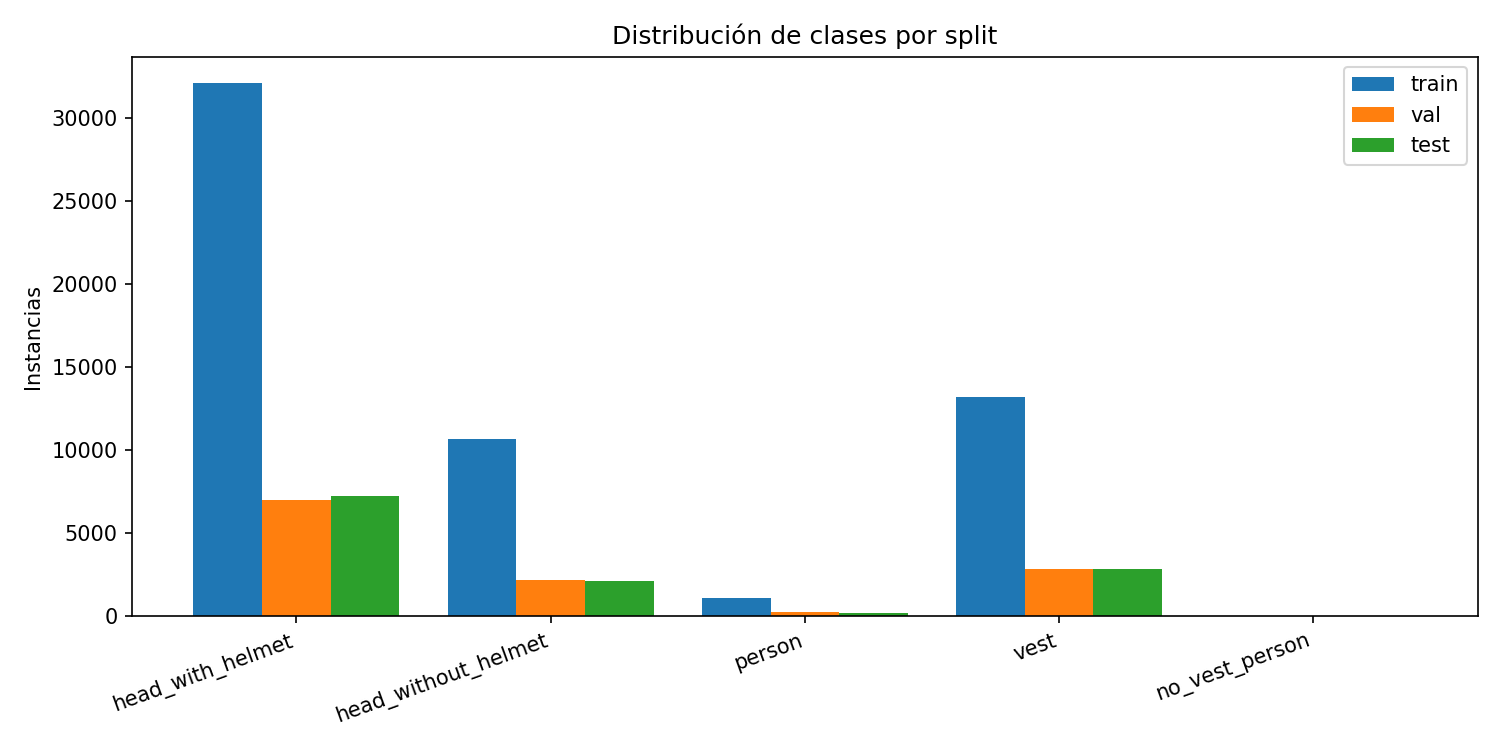
\includegraphics[width=0.85\textwidth]{figures/class_distribution.png}
\caption{Distribución de instancias por clase y por split. Notar la
escasez de \texttt{person} (1.116 train, 2.0\% del total) y la ausencia
total de \texttt{no\_vest\_person} en todos los splits — esta clase se
infiere por reglas en el verificador.}
\label{fig:dist}
\end{figure}

\subsection{Reconocimiento de límites del dataset}

Dos limitaciones se identifican explícitamente:

\begin{enumerate}
    \item \textbf{Clase \texttt{person} muy escasa} (2.0\% de las
    instancias): los tres datasets son detectores centrados en EPP,
    no anotan exhaustivamente el cuerpo completo.
    \item \textbf{\texttt{no\_vest\_person} ausente}: ningún dataset
    aporta esa etiqueta. La ausencia de chaleco se infiere por reglas
    espaciales en el verificador.
    \item \textbf{Anotación parcial no superpuesta}: Hard Hat y SHWD
    anotan solo cabezas; PPE anota solo chalecos. Esta limitación
    se discute en profundidad en la Sección~\ref{sec:hallazgo}.
\end{enumerate}

% ============================================================
\section{Metodología}
% ============================================================

\subsection{Elección del modelo}

Se eligió \textbf{YOLOv8} (Ultralytics) por madurez del tooling,
documentación extensa, compatibilidad probada con Kaggle y excelente
relación costo-beneficio frente a YOLOv9 para un parcial con plazo
definido. Se usó la variante \textbf{YOLOv8s} (small, $\sim$11M parámetros).

\subsection{Configuración base (baseline)}

\begin{table}[h]
\centering
\begin{tabular}{ll}
\toprule
\textbf{Hiperparámetro} & \textbf{Valor} \\
\midrule
Resolución de entrada & 640$\times$640 \\
Epochs & 80 \\
Patience (early stopping) & 20 \\
Optimizador & SGD \\
Learning rate inicial & 0.01 \\
Batch & 16 \\
Mosaic & 1.0 \\
MixUp & 0.0 (desactivado) \\
Random Erasing & 0.0 (desactivado) \\
\bottomrule
\end{tabular}
\caption{Hiperparámetros del baseline.}
\end{table}

\subsection{Experimentos comparativos}

Se diseñaron cuatro experimentos para atacar los tres desafíos del
enunciado. Por restricciones de cuota GPU (Kaggle: 30 h semanales,
$\sim$7--8 h por entrenamiento) se ejecutaron dos:

\begin{table}[h]
\centering
\begin{tabular}{cll}
\toprule
\textbf{Exp} & \textbf{Cambio vs baseline} & \textbf{Objetivo} \\
\midrule
A & Resolución 960 & Mejorar detección de objetos pequeños \\
\textbf{B} & \textbf{mixup=0.15, erasing=0.4} & \textbf{Robustez a oclusión} \\
C & Pesos de clase / oversampling & Atacar desbalance de clases \\
\textbf{D} & \textbf{close\_mosaic=15} & \textbf{Afinar epochs finales} \\
\bottomrule
\end{tabular}
\caption{Experimentos diseñados. B y D se ejecutaron; A y C se descartaron
por costo/beneficio.}
\end{table}

\textbf{A se descartó} por riesgo de timeout en Kaggle ($\sim$12--15 h
estimadas, sobre el límite de 12 h por sesión). \textbf{C se descartó}
porque el problema de \texttt{person} es de \emph{cantidad de datos}
(1.116 train), no de balance: ningún esquema de pesos ``inventa'' más
ejemplos.

\subsection{Decisiones técnicas justificadas}

\textbf{Anchors}: Ultralytics 8.x usa estrategia \emph{anchor-free} con
Distribution Focal Loss. No hay anchors a configurar.

\textbf{Augmentaciones}: estrictamente las nativas de Ultralytics (HSV
jitter, flip horizontal, traslación, escala, mosaic). El Exp. B añadió
Random Erasing y MixUp moderado.

\textbf{Mosaic}: activo durante 65 de 80 epochs en el modelo final
(\texttt{close\_mosaic=15} desactiva en los últimos 15 para afinar con
imágenes en su distribución natural).

\textbf{Resolución}: 640 en todos los experimentos.

% ============================================================
\section{Resultados cuantitativos}
% ============================================================

\subsection{Comparación de experimentos sobre validación}

\begin{table}[h]
\centering
\begin{tabular}{lrrr}
\toprule
\textbf{Clase} & \textbf{Baseline} & \textbf{Exp B} & \textbf{Exp D} \\
\midrule
head\_with\_helmet (mAP@0.5) & 0.978 & 0.978 & \textbf{0.979} \\
head\_without\_helmet (mAP@0.5) & 0.959 & 0.960 & 0.959 \\
vest (mAP@0.5) & 0.987 & 0.986 & 0.986 \\
person (mAP@0.5) & 0.175 & 0.153 & 0.175 \\
\midrule
\textbf{all mAP@0.5} & \textbf{0.775} & 0.769 & \textbf{0.775} \\
\textbf{all mAP@0.5--0.95} & 0.567 & 0.562 & \textbf{0.569} \\
\bottomrule
\end{tabular}
\caption{Comparación de los tres experimentos sobre val. Modelo elegido:
\textbf{Experimento D}.}
\end{table}

\textbf{Hallazgo del Exp. B}: las augmentaciones agresivas (Random
Erasing + MixUp) \emph{no aportaron} mejora en este dataset; degradaron
ligeramente la precisión global ($-0.6$ pp). Hallazgo válido para
reportar honestamente.

\begin{figure}[h]
\centering
\begin{subfigure}{0.48\textwidth}
    \centering
    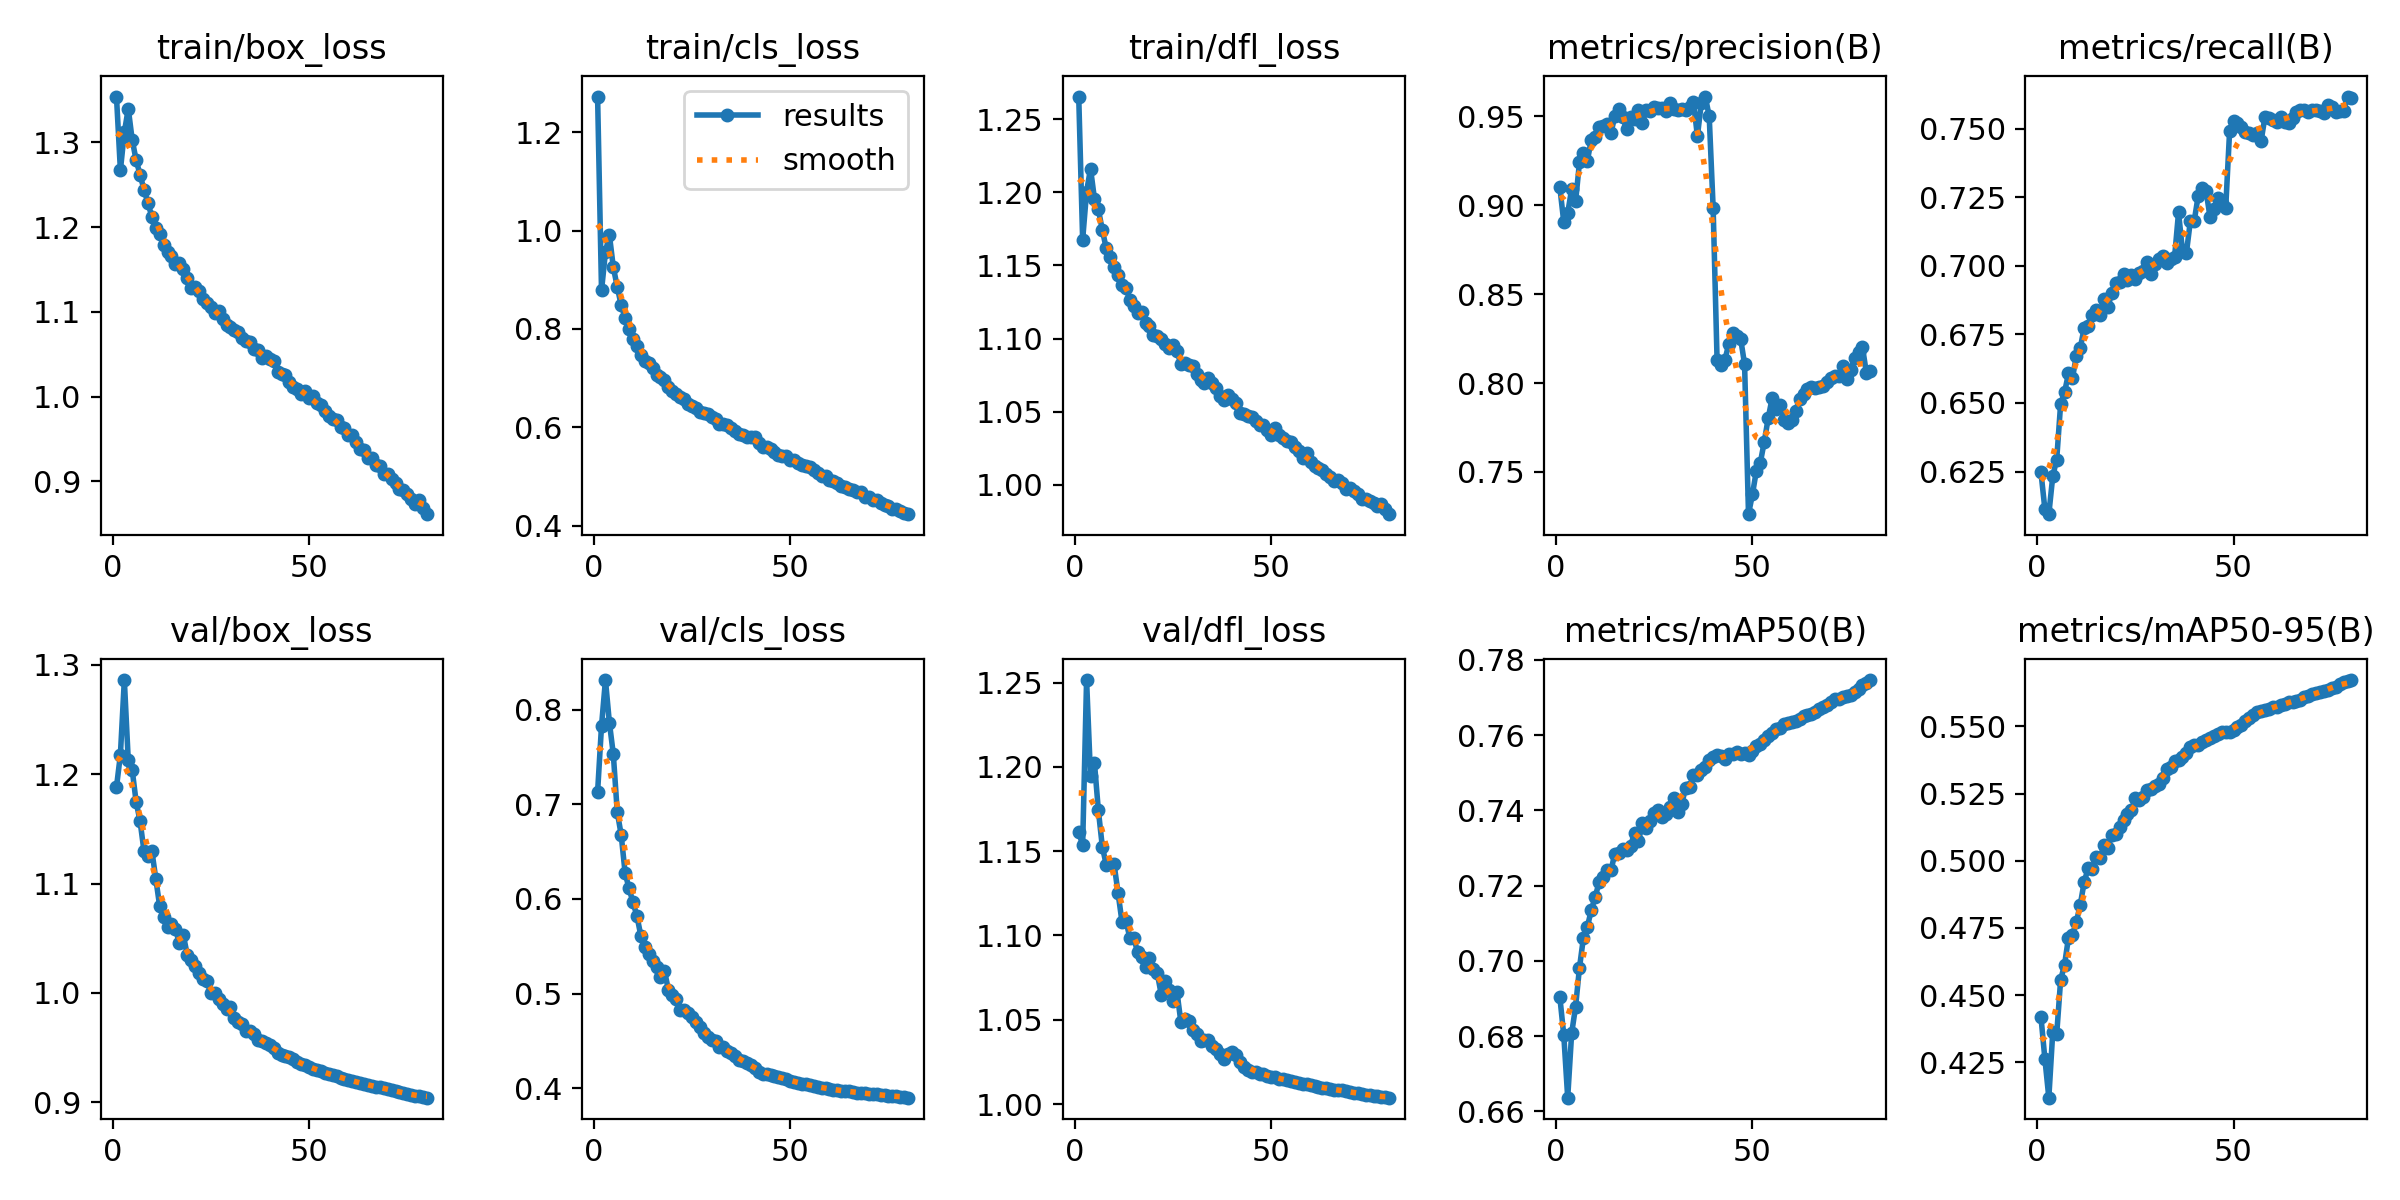
\includegraphics[width=\linewidth]{figures/results_baseline.png}
    \caption{Baseline}
\end{subfigure}
\hfill
\begin{subfigure}{0.48\textwidth}
    \centering
    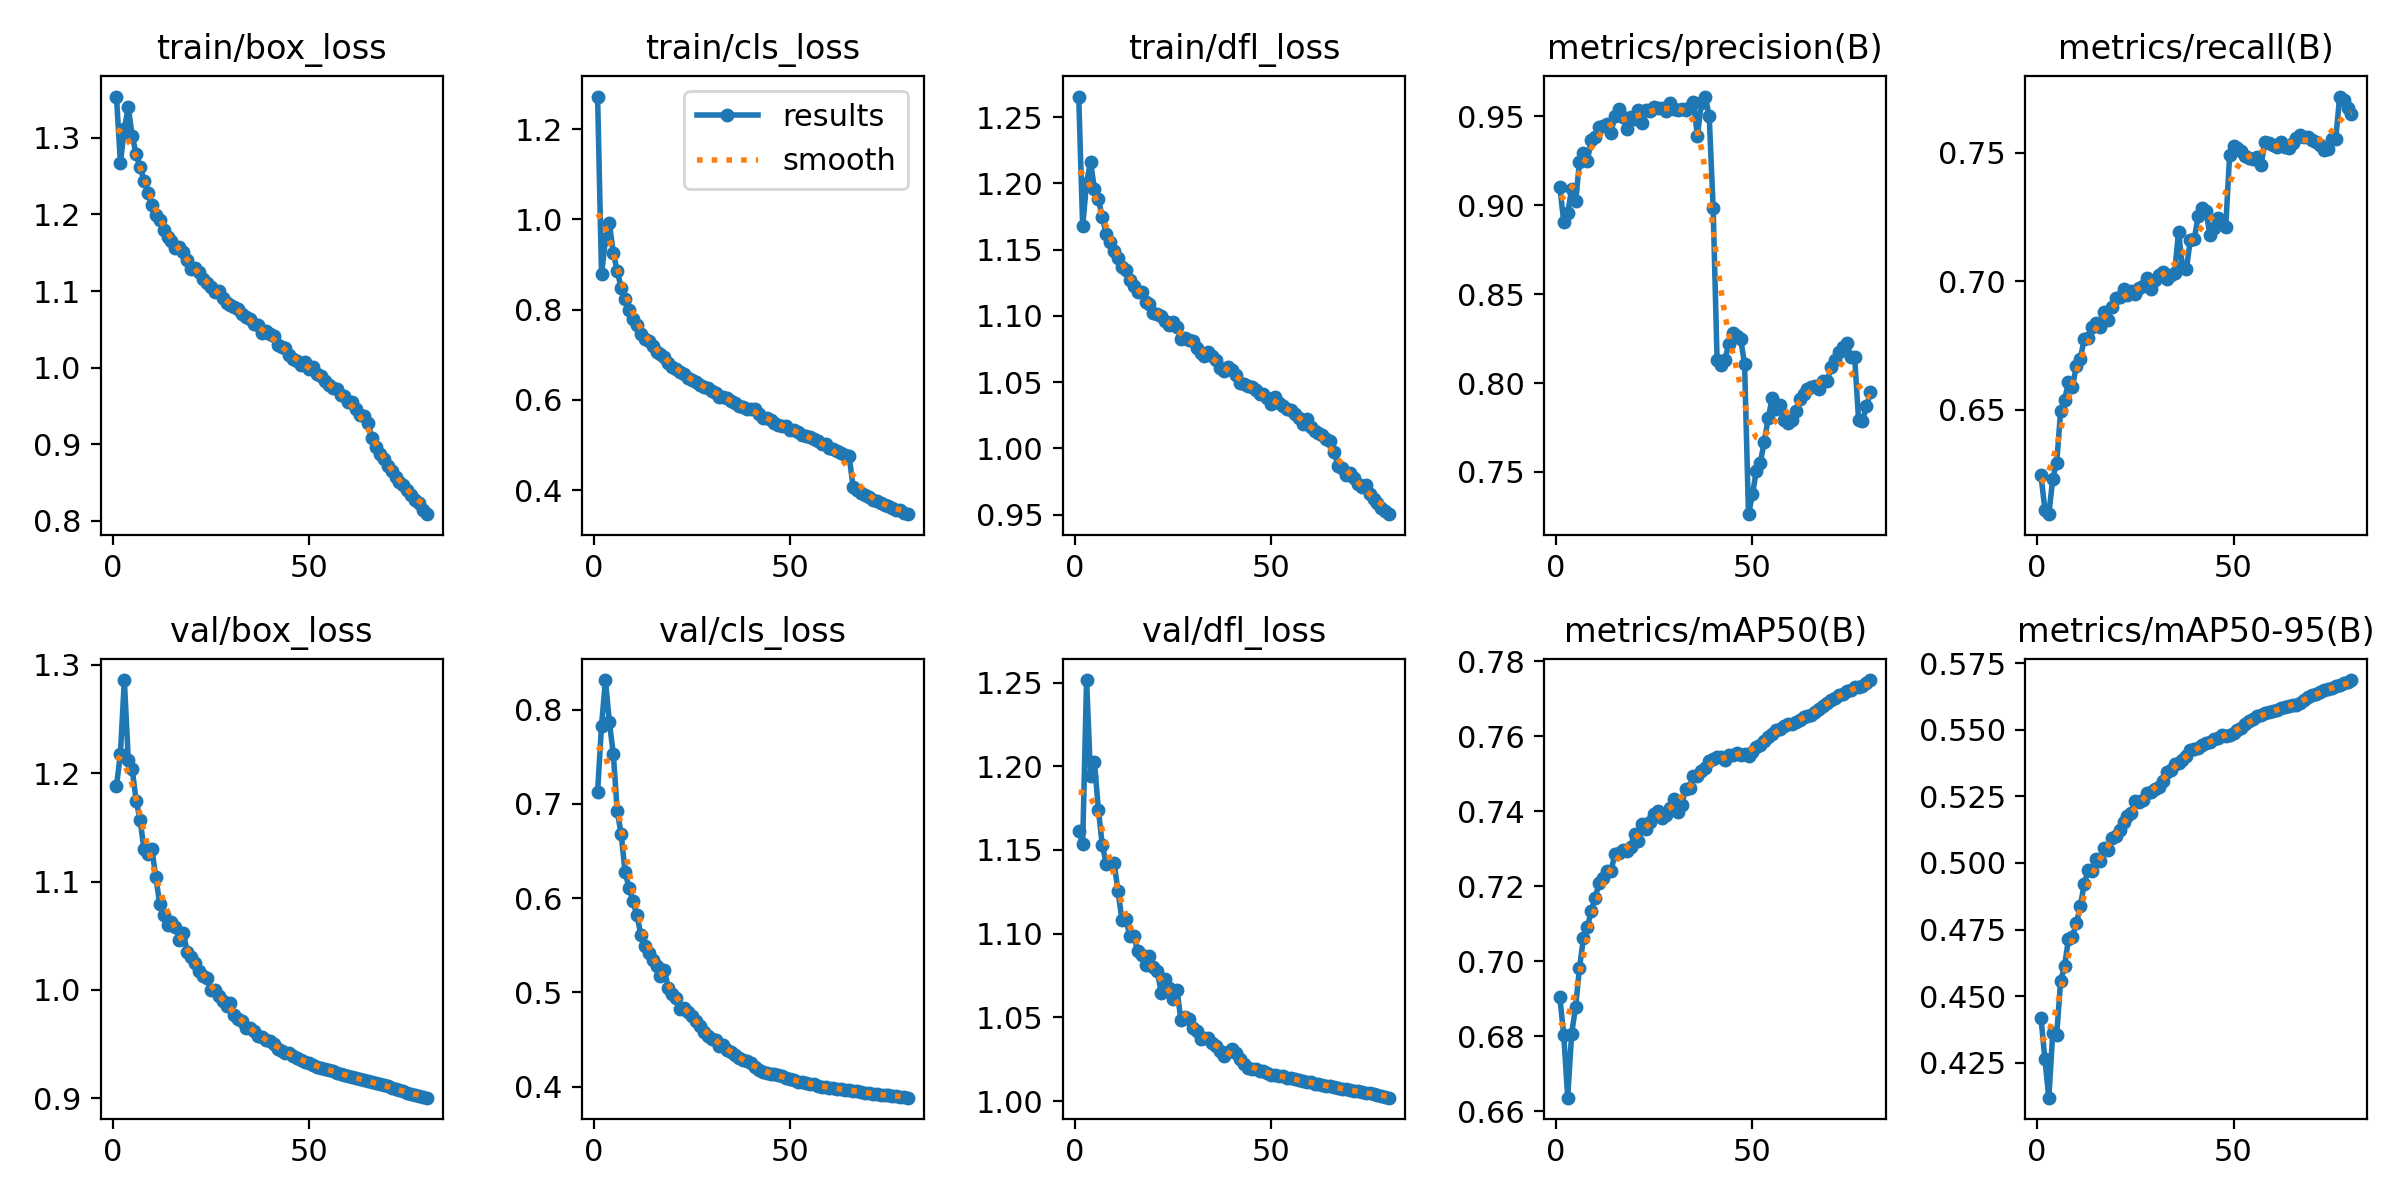
\includegraphics[width=\linewidth]{figures/results_exp_D.png}
    \caption{Exp. D (modelo elegido)}
\end{subfigure}
\caption{Curvas de entrenamiento: pérdidas (train/val) y métricas (mAP,
precision, recall) por epoch. Ambos modelos convergen sin overfitting.}
\end{figure}

\subsection{Evaluación final sobre el conjunto de prueba}

Modelo D evaluado sobre \textbf{3.895 imágenes nunca vistas} durante el
entrenamiento ni la selección de hiperparámetros.

\begin{table}[h]
\centering
\begin{tabular}{lrrrrr}
\toprule
\textbf{Clase} & \textbf{Inst.} & \textbf{Precision} & \textbf{Recall} & \textbf{mAP@0.5} & \textbf{mAP@0.5--0.95} \\
\midrule
head\_with\_helmet & 7.222 & 0.939 & 0.950 & \textbf{0.976} & 0.664 \\
head\_without\_helmet & 2.104 & 0.892 & 0.942 & \textbf{0.947} & 0.646 \\
vest & 2.831 & 0.937 & 0.957 & \textbf{0.984} & 0.837 \\
person & 216 & 0.341 & 0.208 & 0.176 & 0.129 \\
\midrule
\textbf{all} & 12.373 & \textbf{0.777} & \textbf{0.765} & \textbf{0.771} & \textbf{0.569} \\
\bottomrule
\end{tabular}
\caption{Métricas finales del modelo D sobre el test set.}
\label{tab:test}
\end{table}

\begin{figure}[h]
\centering
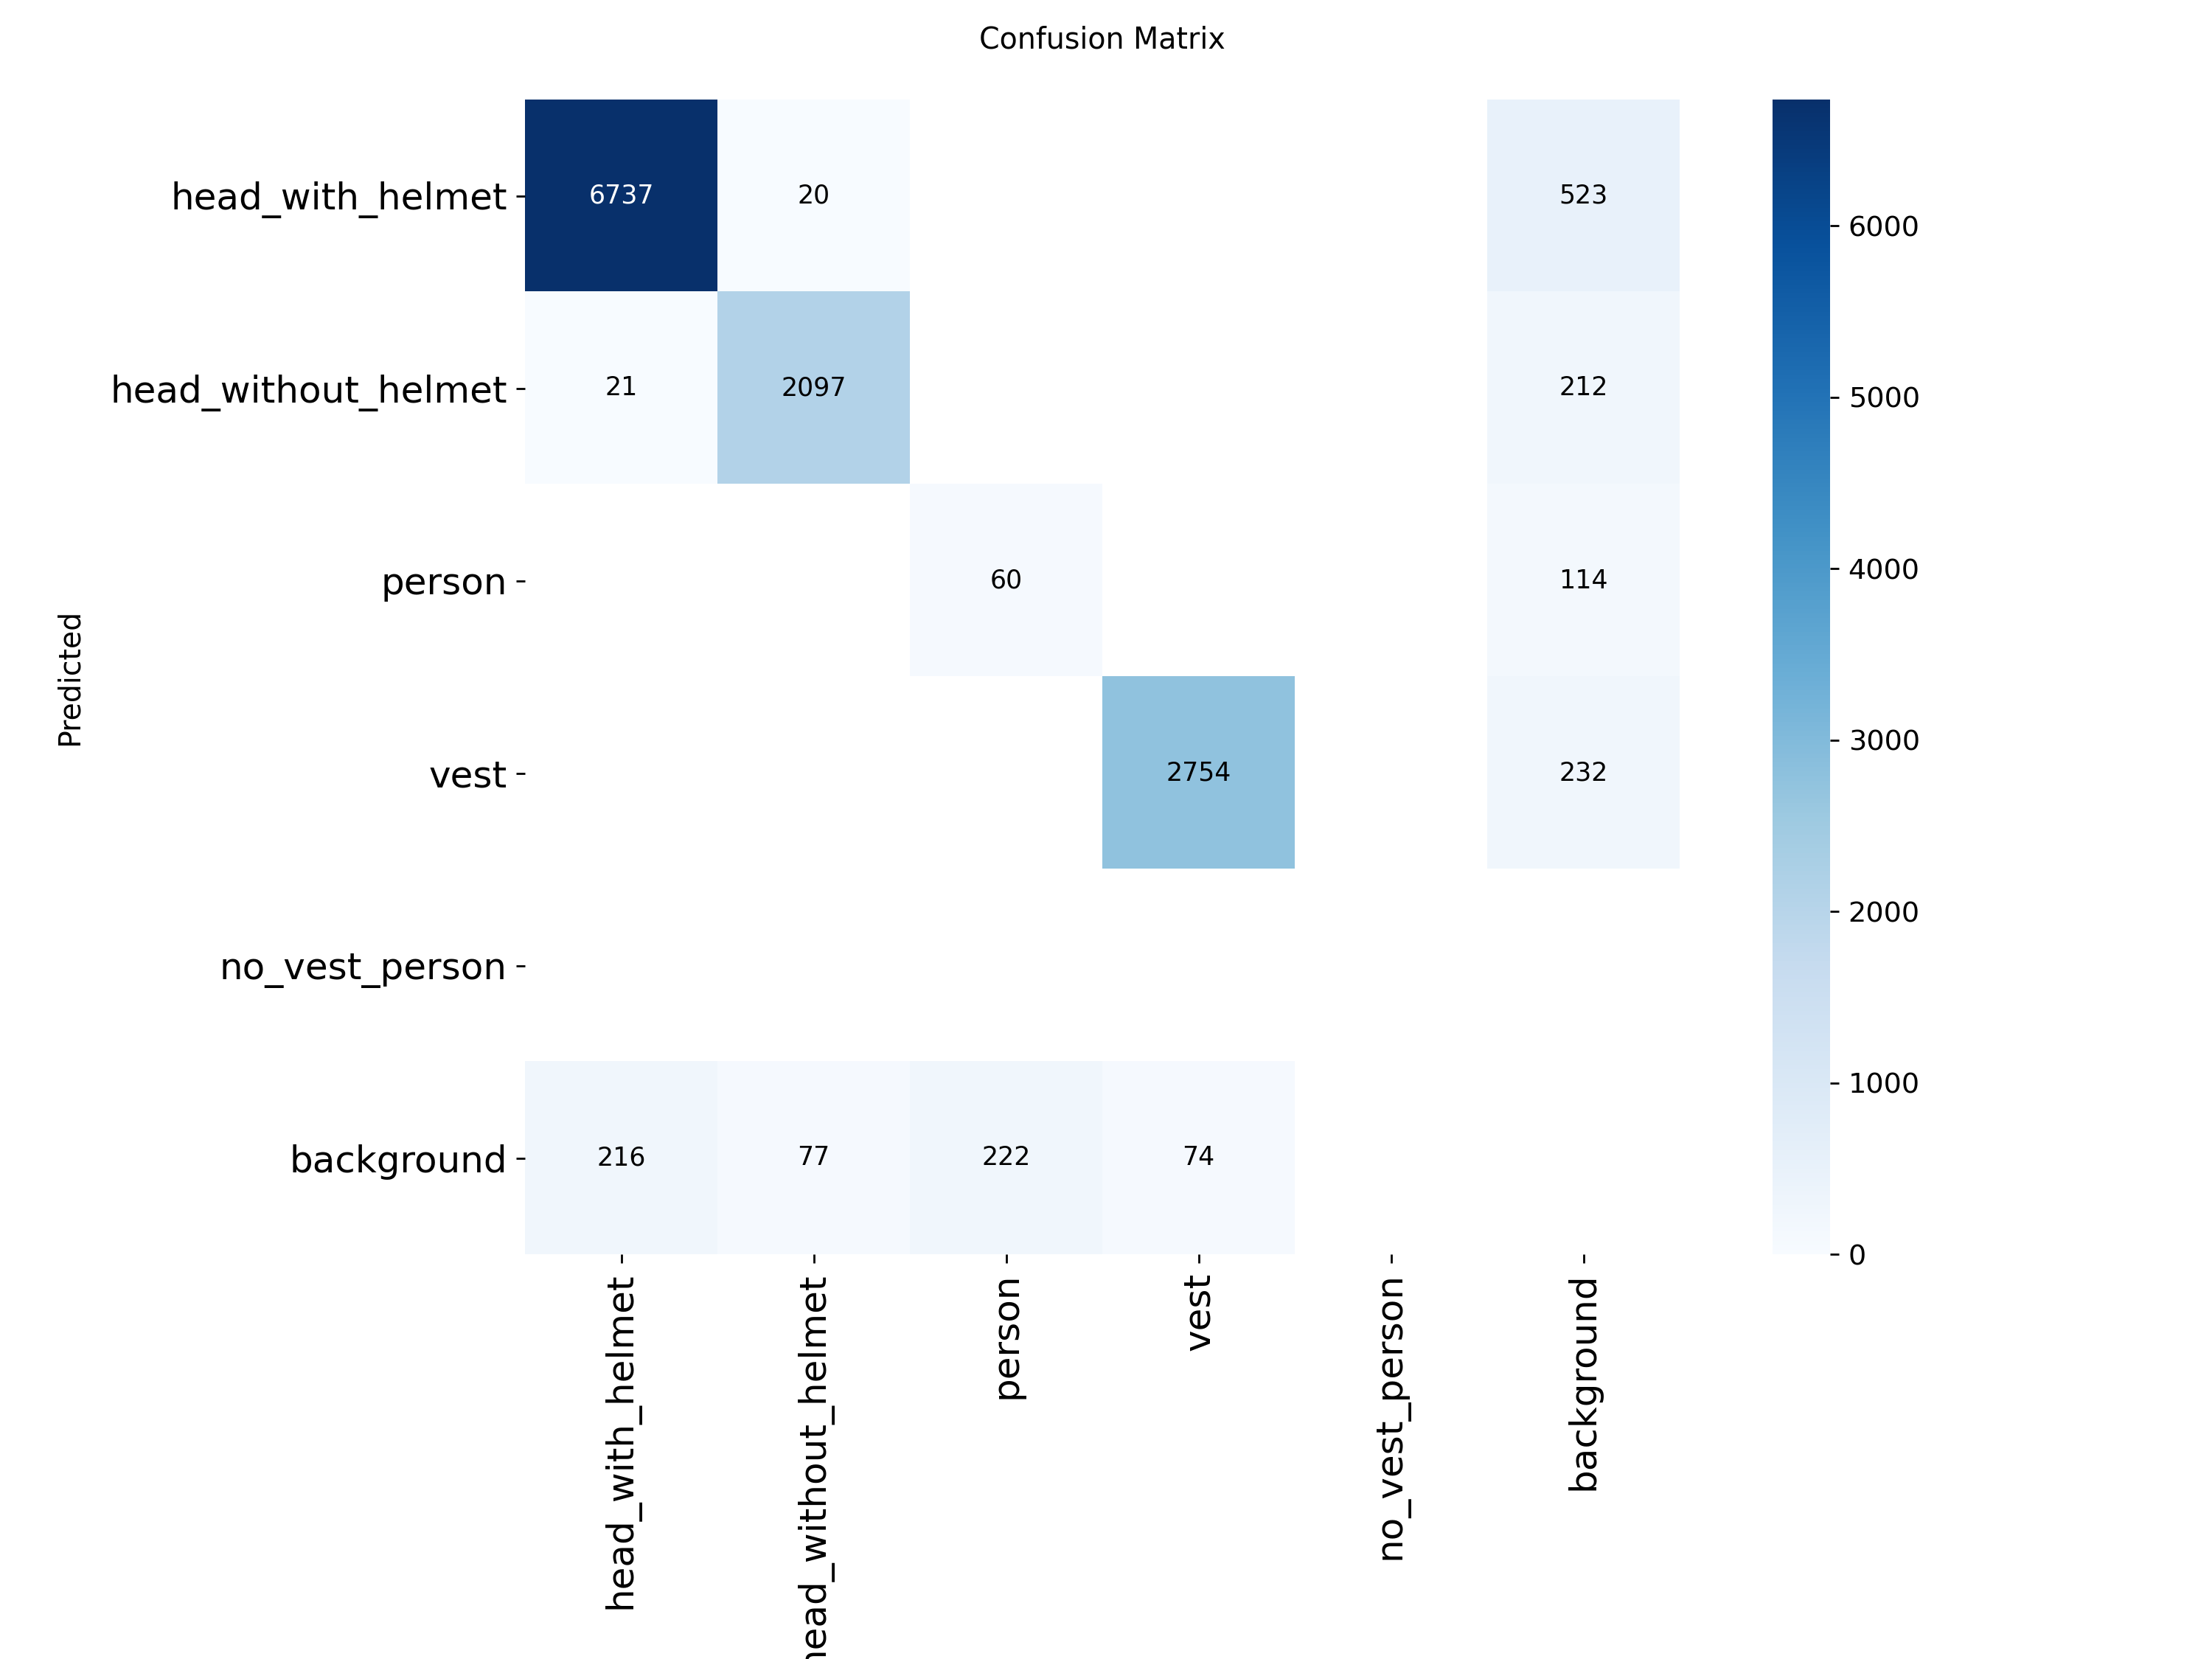
\includegraphics[width=0.7\textwidth]{figures/confusion_exp_D.png}
\caption{Matriz de confusión del modelo D sobre validación. Notar la
diagonal fuerte para las tres clases principales y la confusión casi
inexistente entre clases: los errores caen mayoritariamente en
\emph{background} (falsos negativos o falsos positivos), no en
otra clase.}
\end{figure}

\subsection{Generalización (val vs test)}

\begin{table}[h]
\centering
\begin{tabular}{lrrrl}
\toprule
\textbf{Métrica} & \textbf{Val} & \textbf{Test} & \textbf{$\Delta$} & \textbf{Interpretación} \\
\midrule
mAP@0.5 & 0.775 & 0.771 & $-0.004$ & Sin overfitting \\
mAP@0.5--0.95 & 0.569 & 0.569 & $0.000$ & Idéntico \\
Precision & 0.795 & 0.777 & $-0.018$ & Caída mínima \\
Recall & 0.765 & 0.765 & $0.000$ & Idéntico \\
\bottomrule
\end{tabular}
\caption{Las métricas test son prácticamente idénticas a val. Los splits
estratificados sin fuga funcionaron correctamente.}
\end{table}

\subsection{Análisis de robustez por nivel de oclusión}

Para cada imagen del test se calculó el \textbf{IoU máximo entre cualquier
par de cajas anotadas} y se clasificó en tres niveles.

\begin{table}[h]
\centering
\begin{tabular}{lrrrrr}
\toprule
\textbf{Nivel} & \textbf{n} & \textbf{mAP@0.5} & \textbf{mAP@0.5--0.95} & \textbf{Precision} & \textbf{Recall} \\
\midrule
Bajo (IoU $< 0.15$) & 3.695 & 0.779 & 0.576 & 0.782 & 0.796 \\
Medio (0.15--0.40) & 185 & 0.789 & 0.565 & 0.797 & 0.749 \\
Alto ($\geq$ 0.40) & 15 & 0.704 & 0.512 & 0.783 & 0.623 \\
\midrule
\textbf{Caída bajo $\to$ alto} & — & \textbf{$-7.5$ pp} & $-6.4$ pp & $+0.1$ pp & \textbf{$-17.3$ pp} \\
\bottomrule
\end{tabular}
\caption{Métricas por nivel de oclusión sobre el test set.}
\end{table}

\textbf{Lectura}:
\begin{itemize}
    \item El modelo es \emph{robusto a oclusión leve-media}: \textit{low}
    y \textit{medium} tienen mAP@0.5 prácticamente equivalente.
    \item La oclusión alta sí degrada el desempeño: caída de 7.5 pp en
    mAP@0.5.
    \item \textbf{El recall es la métrica más afectada} ($-17.3$ pp), no
    la precisión. El modelo \emph{pierde detecciones} (no las ve) cuando
    hay oclusión fuerte; las que sí encuentra siguen bien clasificadas.
    Operativamente: en escenas concurridas se podrían perder trabajadores
    no conformes (\emph{falso negativo} crítico para seguridad).
    \item \textbf{Caveat estadístico}: el grupo ``alto'' tiene $n=15$.
    El intervalo de confianza del ``$-7.5$ pp'' es amplio.
\end{itemize}

% ============================================================
\section{Verificador determinista de cumplimiento}
% ============================================================

\subsection{Diseño}

El verificador es un \textbf{módulo Python independiente} que consume las
detecciones de YOLO por fotograma y emite un veredicto por trabajador.
Implementado en \texttt{src/compliance/} con tres archivos:
\texttt{geometry.py}, \texttt{verifier.py}, \texttt{renderer.py}.
Cuenta con \textbf{29 tests unitarios pytest} sobre escenarios sintéticos.

\subsection{Estrategia de asociación: cabeza-ancla}

El diseño inicial usaba \texttt{person} como ancla. En evaluación
cualitativa este diseño falló porque la clase \texttt{person} tiene
recall del 17\% sobre val.

Se reescribió la lógica como \textbf{cabeza-ancla}: para cada cabeza
detectada, se busca un chaleco debajo con alineación horizontal
razonable. Si existe un \texttt{person} que contiene la cabeza, se usa
solo para enriquecer el rendering. Esta versión opera correctamente con
las detecciones reales del modelo.

\subsection{Lógica de veredicto}

\begin{table}[h]
\centering
\begin{tabular}{ll}
\toprule
\textbf{Detecciones asociadas a un trabajador} & \textbf{Veredicto} \\
\midrule
cabeza con casco + chaleco debajo & \textbf{CONFORME} \\
cabeza con casco, sin chaleco & NO\_CONFORME (``chaleco\_no\_visible'') \\
cabeza sin casco & NO\_CONFORME (``casco\_ausente'') \\
chaleco huérfano sin cabeza visible & INDETERMINADO (``cabeza\_no\_visible'') \\
\bottomrule
\end{tabular}
\caption{Lógica de decisión del verificador determinista.}
\end{table}

\begin{figure}[h]
\centering
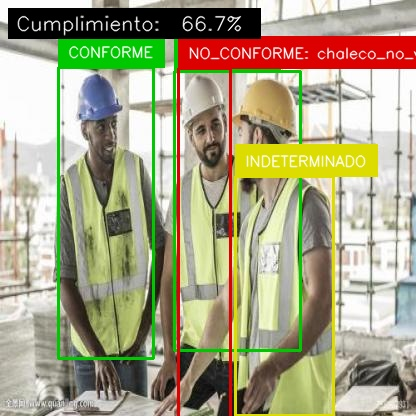
\includegraphics[width=0.75\textwidth]{figures/verifier_imagen.jpg}
\caption{Ejemplo de salida del verificador sobre una imagen del val set:
3 trabajadores detectados. Bbox verde = CONFORME (casco azul + chaleco
amarillo asociados), rojo = NO\_CONFORME, amarillo = INDETERMINADO
(chaleco sin cabeza asociada). Tasa de cumplimiento del fotograma: 66.7\%.}
\end{figure}

\subsection{Hallazgo principal: sesgo de etiquetado entre datasets}
\label{sec:hallazgo}

Sobre 300 imágenes val analizadas con el modelo D:

\begin{table}[h]
\centering
\begin{tabular}{lr}
\toprule
\textbf{Categoría} & \textbf{\%} \\
\midrule
Solo \texttt{head\_with\_helmet} detectado & 49.0\% \\
Solo \texttt{head\_without\_helmet} detectado & 7.3\% \\
Solo \texttt{vest} detectado & 40.3\% \\
\textbf{\texttt{head} + \texttt{vest} (compatible con CONFORME)} & \textbf{3.3\%} \\
\bottomrule
\end{tabular}
\caption{El modelo D casi nunca firma cabeza y chaleco en la misma
imagen ($\sim$3\%). Causa: SHWD/Hard Hat anotan solo cabezas, PPE
anota solo chalecos; el modelo aprendió la correlación ``estilo de
imagen $\to$ clases visibles''.}
\end{table}

\textbf{Esta es una limitación del dataset, no del verificador.} Para
producción se recomienda re-entrenar sobre un dataset con anotación
completa por trabajador (ej. \emph{Construction Site Safety}, clases
Hardhat + Safety Vest + Person en cada imagen).

% ============================================================
\section{Demostración en video}
% ============================================================

\subsection{Material}

Se procesó un video de obra real \textbf{no visto durante el
entrenamiento}: una cuadrilla colombiana vertiendo concreto desde un
camión Argos en una calle urbana. 25.8 segundos a 30 fps (773 frames)
en 1920$\times$1080.

\subsection{Configuración y resultados}

Modelo: \texttt{runs\_outputs/exp\_D/best.pt}. Resolución de inferencia:
1280 (subida desde el 640 de entrenamiento para detectar cabezas, que
son objetos chicos). Umbral de confianza: 0.15.

\begin{table}[h]
\centering
\begin{tabular}{lr}
\toprule
\textbf{Veredicto} & \textbf{Cantidad sobre 773 frames} \\
\midrule
CONFORME & 861 \\
NO\_CONFORME & 2.600 \\
INDETERMINADO & 1.309 \\
\midrule
\textbf{Tasa de cumplimiento} & \textbf{24.9\%} \\
\bottomrule
\end{tabular}
\caption{Veredictos agregados del modelo D sobre el video demo.}
\end{table}

\begin{figure}[h]
\centering
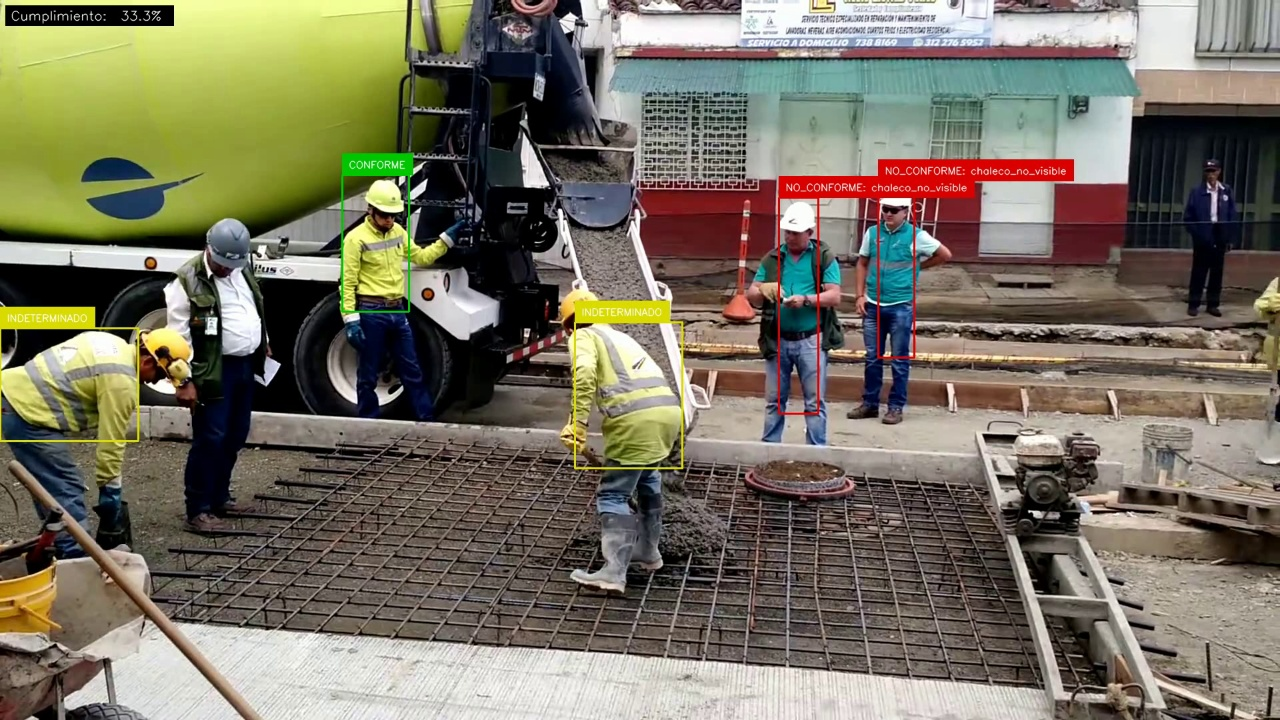
\includegraphics[width=0.85\textwidth]{figures/demo_modelo_D.jpg}
\caption{Fotograma del video demo procesado con el modelo D. Verde =
CONFORME (casco + chaleco asociados), rojo = NO\_CONFORME (con razón
explícita), amarillo = INDETERMINADO (chaleco sin cabeza visible).
Tasa de cumplimiento del fotograma: 33.3\%.}
\end{figure}

\subsection{Archivo del video}

El video anotado completo está disponible localmente como
\texttt{demo\_video/video03\_annotated\_v2.mp4} (114 MB). Para
reproducirlo:

\begin{lstlisting}[language=bash,basicstyle=\ttfamily\small]
python -m src.run_video \
  --weights runs_outputs/exp_D/best.pt \
  --video demo_video/video03p.mp4 \
  --out demo_video/video03_annotated_v2.mp4 \
  --conf 0.15 --imgsz 1280
\end{lstlisting}

\subsection{Validación experimental complementaria}

Para verificar si la alta proporción de INDETERMINADO se debía al
\textbf{pipeline} o al \textbf{dataset de entrenamiento}, se ejecutó
el mismo pipeline sustituyendo el modelo D por un modelo YOLOv8m
externo entrenado sobre un dataset con anotación completa por
trabajador (10 clases incluyendo Hardhat, NO-Hardhat, Safety Vest,
NO-Safety Vest, Person). \textbf{El verificador y el renderer no se
modificaron}; solo se remapean las clases del modelo externo a la
taxonomía unificada antes de pasar al verificador.

\begin{table}[h]
\centering
\begin{tabular}{lrrr}
\toprule
\textbf{Métrica} & \textbf{Modelo D nuestro} & \textbf{Modelo externo} & \textbf{Ratio} \\
\midrule
CONFORME & 861 & 2.287 & \textbf{2.66$\times$} \\
NO\_CONFORME & 2.600 & 7.221 & \textbf{2.78$\times$} \\
INDETERMINADO & 1.309 & 397 & \textbf{0.30$\times \downarrow$} \\
Veredictos determinados & 3.461 & 9.508 & \textbf{2.75$\times$} \\
INDETERMINADO sobre total & 27.4\% & \textbf{4.0\%} & $-85\%$ \\
Tasa cumplimiento (CONF/det.) & 24.9\% & 24.0\% & similar \\
\bottomrule
\end{tabular}
\caption{Validación experimental: el modelo externo produce 2.75$\times$
más veredictos definitivos. La diferencia confirma que el cuello de
botella es el dataset combinado, no el pipeline.}
\end{table}

\begin{figure}[h]
\centering
\begin{subfigure}{0.48\textwidth}
    \centering
    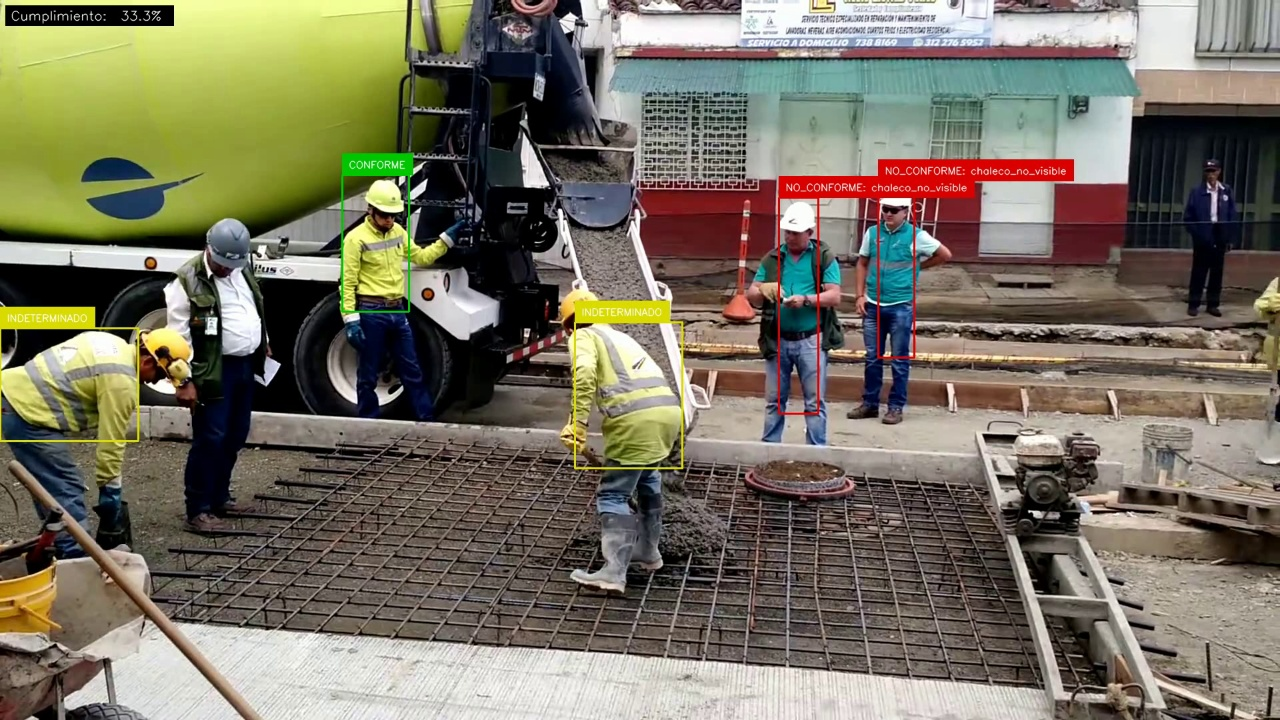
\includegraphics[width=\linewidth]{figures/demo_modelo_D.jpg}
    \caption{Nuestro modelo D}
\end{subfigure}
\hfill
\begin{subfigure}{0.48\textwidth}
    \centering
    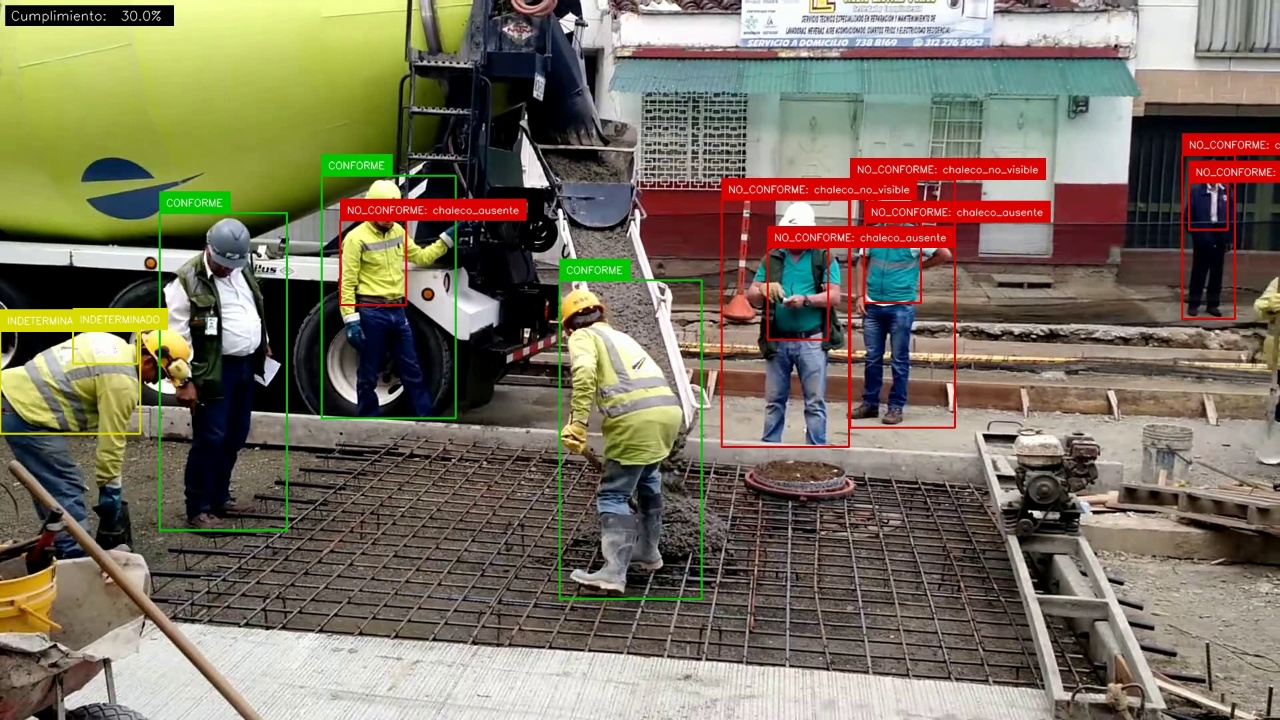
\includegraphics[width=\linewidth]{figures/demo_externo.jpg}
    \caption{Modelo externo}
\end{subfigure}
\caption{Mismo frame del video procesado por ambos modelos. El modelo
externo (derecha) detecta simultáneamente cabezas y chalecos en muchos
más trabajadores, permitiendo al verificador emitir muchos más
veredictos definitivos (verdes y rojos).}
\end{figure}

\textbf{Aclaración de honestidad académica}: el modelo externo no es
producto de este trabajo. Se usó únicamente como referencia experimental
para validar el diagnóstico. El modelo principal entregado sigue siendo
el Experimento D entrenado en este parcial.

% ============================================================
\section{Implicaciones éticas}
% ============================================================

\subsection{Balance entre falsos negativos y falsos positivos}

Los dos tipos de error tienen costos asimétricos:

\begin{itemize}
    \item \textbf{Falso negativo} (no detectar a un trabajador sin EPP):
    el caso queda sin reportar, el trabajador permanece en riesgo. Daño
    humano potencial y responsabilidad legal.
    \item \textbf{Falso positivo} (marcar como no conforme a un trabajador
    conforme): sanción injusta, erosión de confianza en el sistema, posible
    sabotaje.
\end{itemize}

\textbf{En seguridad ocupacional, el falso negativo es típicamente más
costoso} que el falso positivo, porque el riesgo de daño físico es
asimétrico. Sin embargo, una tasa alta de falsos positivos también
compromete el sistema: si los trabajadores aprenden que ``se equivoca
seguido'', dejarán de confiar incluso cuando acierte.

\textbf{Implicación para el umbral operativo}: el umbral de confianza
del clasificador no debe elegirse maximizando el mAP global, sino
considerando el costo asimétrico de los errores. Una recomendación
práctica es elegir el umbral que maximiza recall sobre las clases
críticas (\texttt{head\_without\_helmet}, \texttt{no\_vest\_person})
sujeto a un techo de falsos positivos tolerables.

\textbf{Implicación para el verificador}: el estado INDETERMINADO es
un mecanismo de seguridad importante. El sistema no debe \emph{inventar
veredictos} cuando no tiene evidencia suficiente; debe escalar la
decisión a un humano. Esto es lo que hace el verificador propuesto.

\subsection{Privacidad de los trabajadores}

Un sistema que graba continuamente plantea cuestiones serias:

\begin{itemize}
    \item \textbf{Vigilancia continua}: el monitoreo permanente puede
    generar estrés y desincentivar el reporte voluntario de incidentes.
    \item \textbf{Uso secundario de las imágenes}: las imágenes pueden
    reutilizarse para fines no acordados (evaluación de desempeño,
    identificación en otros contextos).
    \item \textbf{Consentimiento informado}: los trabajadores deben
    saber qué se graba, con qué propósito y por cuánto tiempo. El
    consentimiento bajo coerción laboral no es válido.
\end{itemize}

\textbf{Recomendaciones operativas}: anonimización de rostros a nivel
de pipeline, retención mínima necesaria, acceso restringido por roles,
auditoría de uso. El sistema técnico desarrollado \emph{no} implementa
estas medidas; son necesarias para un despliegue ético.

\subsection{Sesgos introducidos por la distribución de los datos}

Los tres datasets utilizados tienen sesgos identificables:

\begin{itemize}
    \item \textbf{Sesgo geográfico}: los datasets de Roboflow suelen estar
    dominados por imágenes de obras en China, EE.UU. y Europa. Trabajadores
    con vestimenta tradicional o herramientas locales pueden estar
    subrepresentados.
    \item \textbf{Sesgo demográfico}: la distribución de género, edad y
    etnicidad de los trabajadores en los datasets no se reportó ni se
    auditó en este trabajo. Se reconoce explícitamente como limitación.
    \item \textbf{Sesgo de condiciones de captura}: iluminación diurna,
    clima despejado, ángulos fijos. El modelo puede fallar con luz tenue,
    lluvia o cámaras móviles.
\end{itemize}

\textbf{Implicación}: las métricas reportadas (mAP@0.5 = 0.771 en test)
son \emph{válidas para la distribución del test}, no son garantía de
desempeño equivalente en condiciones de despliegue distintas. Para
despliegue real debería hacerse un piloto controlado en el sitio
objetivo, con re-evaluación.

% ============================================================
\section{Limitaciones y trabajo futuro}
% ============================================================

\subsection{Limitaciones reconocidas}

\begin{enumerate}
    \item \textbf{Sesgo de etiquetado entre datasets}: solo el 3.3\%
    de las imágenes val tiene cabeza y chaleco detectados
    simultáneamente.
    \item \textbf{Clase \texttt{person} escasa}: 1.116 instancias en
    train, mAP@0.5 $\approx$ 0.18 sobre test.
    \item \textbf{No se evaluó el Experimento A (resolución 960)} por
    restricción de tiempo de cómputo en Kaggle.
    \item \textbf{Grupo ``oclusión alta'' estadísticamente débil}
    ($n=15$ imágenes).
    \item \textbf{Sin auditoría de sesgos demográficos} sobre los
    datasets.
    \item \textbf{Sin tracking temporal}: cada frame se procesa
    independientemente.
\end{enumerate}

\subsection{Trabajo futuro}

\begin{itemize}
    \item Dataset con anotación completa por trabajador
    (\emph{Construction Site Safety} con Hardhat + Safety Vest + Person
    en cada imagen).
    \item Modelo más grande: YOLOv8m o YOLOv9.
    \item Resolución 960 o 1280 para mejorar objetos pequeños.
    \item Tracking temporal (ByteTrack) para estabilizar veredictos
    entre frames.
    \item Calibración del umbral operativo según costo asimétrico.
    \item Detección de arnés para trabajos en altura.
\end{itemize}

% ============================================================
\section{Conclusiones}
% ============================================================

\begin{enumerate}
    \item Se entrenó un detector YOLOv8s con \textbf{mAP@0.5 = 0.771}
    sobre test no visto, con desempeño excelente en las tres clases
    críticas (cabezas con/sin casco y chalecos, todas $\geq$ 0.947).

    \item \textbf{El modelo generaliza correctamente}: las métricas
    test son prácticamente idénticas a val ($-0.4$ pp), validando los
    splits estratificados de la Fase 1.

    \item \textbf{El verificador determinista funciona}: 29 tests
    unitarios pasando + inspección cualitativa sobre val y video real
    confirmaron que la lógica es correcta.

    \item La principal \textbf{limitación operativa es del modelo, no
    del verificador}: el sesgo de etiquetado entre los tres datasets
    hace que solo el 3.3\% de las imágenes tengan cabeza y chaleco
    detectados simultáneamente. Esto se documentó cuantitativamente
    y \textbf{se validó experimentalmente} comparando contra un modelo
    externo: ese modelo produce 2.75$\times$ más veredictos definitivos
    sobre la misma escena.

    \item El sistema \textbf{expone honestamente su incertidumbre}
    mediante el estado INDETERMINADO. No inventa veredictos cuando le
    falta evidencia.

    \item La sección ética identifica tres ejes críticos: asimetría de
    errores, privacidad y sesgos del dataset. El sistema técnico no
    resuelve estos ejes por sí solo; requieren políticas operativas y
    de gobernanza.
\end{enumerate}

% ============================================================
\appendix
\section{Reproducibilidad}
% ============================================================

\subsection{Estructura del repositorio}

\begin{lstlisting}[language=bash,basicstyle=\ttfamily\footnotesize]
epp-yolo-compliance/
├── configs/                 # data.yaml, hyp_*.yaml, class_mapping.yaml
├── data/                    # gitignored (datasets descargados manualmente)
├── notebooks/kaggle/        # 8 notebooks orquestadores
├── reports/                 # tablas, figuras, informe
├── src/
│   ├── analysis/            # análisis de oclusión
│   ├── compliance/          # geometría + verificador + renderer
│   └── data/                # remap, splits, validación
├── tests/                   # 39 tests pytest
├── pyproject.toml
├── requirements.txt
└── README.md
\end{lstlisting}

\subsection{Notebooks de entrenamiento y evaluación}

\begin{table}[h]
\centering
\begin{tabular}{llr}
\toprule
\textbf{Notebook} & \textbf{Propósito} & \textbf{Tiempo} \\
\midrule
\texttt{01\_baseline\_train} & Baseline YOLOv8s @ 640 & $\sim$7.3 h \\
\texttt{03\_exp\_B\_augmentation} & Random Erasing + MixUp & $\sim$7.9 h \\
\texttt{05\_exp\_D\_close\_mosaic} & close\_mosaic=15 (final) & $\sim$7.2 h \\
\texttt{07\_test\_evaluation} & Eval sobre test set & $\sim$4 min \\
\texttt{08\_occlusion\_analysis} & mAP por nivel de oclusión & $\sim$5 min \\
\bottomrule
\end{tabular}
\caption{Notebooks de Kaggle. Modelo final: notebook 05 + 07.}
\end{table}

\subsection{Pipeline de inferencia local}

\begin{lstlisting}[language=bash,basicstyle=\ttfamily\small]
# Inferencia + verificador sobre imágenes
python -m src.run_pipeline \
  --weights runs_outputs/exp_D/best.pt \
  --images data/processed/images/test \
  --out reports/figures/demo --n 20

# Inferencia + verificador sobre video
python -m src.run_video \
  --weights runs_outputs/exp_D/best.pt \
  --video demo_video/video03p.mp4 \
  --out demo_video/video03_annotated_v2.mp4 \
  --conf 0.15 --imgsz 1280
\end{lstlisting}

\subsection{Artefactos publicados}

\begin{itemize}
    \item \textbf{Código}: \url{https://github.com/PercyTechX/epp-yolo-compliance}
    \item \textbf{Release del modelo final}:
    \url{https://github.com/PercyTechX/epp-yolo-compliance/releases/tag/v1.0}
    \item \textbf{Dataset remapeado (Kaggle)}:
    \texttt{jpnazariop/epp-yolo-processed}
    \item \textbf{Pesos del modelo final (Kaggle)}:
    \texttt{jpnazariop/epp-yolo-exp-d-weights}
\end{itemize}

\end{document}
